\section{Modelo de Arquitetura} 
Este capítulo começa por introduzir o \textit{stack} tecnológico sobre o qual o projeto foi desenvolvido. O mesmo contém também um secção atribuída a cada módulo do projeto e por fim refere as tecnologias usadas no mesmo.
\par \medskip

O modelo de arquitetura do nosso projeto, apresentado na Figura 4, é constituído por três módulos principais: uma REST API, e duas aplicações cliente: uma orientada à plataforma \textit{mobile} Android e outra desenvolvida para ser usada num \textit{browser}. \par \medskip

Tendo em conta os módulos constituintes do projeto, o desenvolvimento do mesmo seguirá o \textit{stack} MEAN \textit{stack}~\cite{mean_stack_explained} (MongoDB, Express.js, Angular, Node.js), alternando a tecnologia utilizada para desenvolver o \textit{front-end} para React em vez de Angular (também conhecido pelo MERN \textit{stack}, referido na Figura 3). Foi escolhido este \textit{standard} pelas seguintes razões:
\begin{itemize}
	\item familiaridade dos autores com algumas destas tecnologias (como Express.js e Node.js);
	\item \textit{stack} utilizado no desenvolvimento de múltiplas aplicações, o que leva a existência de uma grande quantidade de recursos, como documentação e exemplos;
	\item todas estas tecnologias têm em comum características que as tornam apelativas de usar conjuntamente, como por exemplo o facto da utilização de JSON ser transversal entre todas;
	\item todas as ferramentas associadas a esta pilha tecnológica são \textit{open-source}.
\end{itemize}

\begin{figure}[h]
	\centering
	
\includegraphics[scale=.35]{mern2}
	\caption{Tecnologias do \textit{stack} MERN (MongoDB, Express.js, React.js, Node.js)}
\end{figure}

Relativamente à API, esta estabelecerá \textit{endpoints} onde será possível executar pedidos HTTP de maneira a suportar autenticação e operações na infraestrutura (criação de perfil, “seguimento” de organização, inscrição em ação de voluntariado, etc.), constituindo o \textit{back-end} do projeto.
\par \medskip

Relativamente ao \textit{front-end}, foram desenvolvidas duas aplicações cliente: 
\begin{itemize}
	\item um cliente \textit{mobile}, para a plataforma Android, usado pelos voluntários. Nesta interface será possível efetuar por parte do utilizador as operações de uso da plataforma usuais: criação de um perfil, visionamento de um \textit{feed} de \textit{posts} efetuados pelas organizações seguidas, entre outras;
	\item um cliente \textit{browser}. Esta aplicação é direcionada às organizações e terá a finalidade de permitir às mesmas realizar \textit{posts}, criar e gerir ações de voluntariado, etc.;
\end{itemize}

\begin{figure}[h]
	\centering
	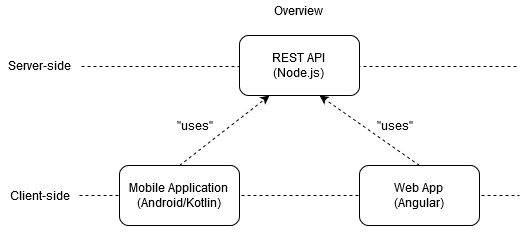
\includegraphics[scale=.8]{architecture}
	\caption{Modelo de arquitetura}
\end{figure}


\subsection{REST API}
A REST API, definida como primeira fase do projeto, constituirá o \textit{server-side} do mesmo. É pretendido que este módulo seja completamente independente dos outros, tendo como responsabilidade trabalhar como fonte de dados para os outros componentes (\textit{client-side}). \par \medskip 

A tecnologia utilizada para desenvolver este componente foi Node.js em conjunto com vários \textit{packages} do NPM (\textit{node package manager}), como o Express e o Passport. Esta escolha é justificada por múltiplas razões:
\begin{itemize}
	\item domínio dos autores na linguagem Javascript e em vários módulos do NPM;
	\item popularidade da ferramenta, algo que simplifica o processo de desenvolvimento do componente devido à existência de grande quantidade de recursos sobre a mesma;
	\item existência de suporte neste meio de execução de ferramentas para auxiliar o acesso à base de dados escolhida.
\end{itemize}
\par \medskip

O servidor será também responsável por hospedar a base de dados, que irá funcionar no motor MongoDB. A escolha deste serviço foi efetuada devido à fácil integração do mesmo com Node.js e devido ao facto deste ter um modelo de dados baseado em documentos JSON, algo que simplifica a inserção e pesquisa sobre os mesmos.
\par \medskip

\subsection{Aplicação \textit{Mobile}}
A aplicação \textit{mobile} será desenvolvida para a plataforma Android em Kotlin. A mesma irá seguir os princípios definidos pelo Android Jetpack, que disponibiliza ferramentas e bibliotecas que auxiliam o desenvolvimento da aplicação. As razões que levaram a esta decisão foram:
\begin{itemize}
	\item familiaridade dos autores com esta linguagem de programação e ferramentas (Android Jetpack);
	\item a nível de quota de mercado dos sistemas operativos de dispositivos móveis, o Android é o mais prevalente;
	\item o Kotlin é uma das linguagens oficiais para desenvolvimento de aplicações móveis para Android.
\end{itemize}

\subsection{Aplicação \textit{Web}}
A aplicação \textit{web} será desenvolvida em React~\cite{angular_vs_react}. Esta tecnologia foi escolhida devido a:

\begin{itemize}
	\item familiaridade dos autores com esta ferramenta;
	\item quota de mercado (relativamente às \textit{frameworks} de Javascript utilizadas para o desenvolvimento de aplicações \textit{web}) significativa, sendo atualmente a tecnologia mais usada~\cite{angular_vs_react};
	\item fácil integração com as outras ferramentas do projeto.
\end{itemize}

\subsection{Tecnologias e ferramentas}
As seguintes tecnologias irão ser utilizadas durante o desenvolvimento do projeto:
\begin{itemize}
	\item \textbf{Javascript}: Principal linguagem para programação \textit{client-side} em \textit{browsers}; Esta é tipicamente utilizada em conjunto com ferramentas como o HTML e CSS para implementar a funcionalidade de uma página \textit{web};
	\item \textbf{Node.js}: Interpretador e ambiente de execução para Javascript normalmente utilizado para executar código sem ser num cliente \textit{browser};
	\item \textbf{NPM}: \textit{package manager} do Javascript/Node.js;
	\item \textbf{Express}: \textit{web framework} para Node.js. Auxilia o processo de \textit{routing} e definição de \textit{endpoints}, encapsulando aspetos do HTTP, para tornar mais fácil o desenvolvimento de \textit{Web} APIs;
	\item \textbf{Passport}: \textit{Middleware} de autenticação usado em conjunto com o Express para simplificar o processo de autenticação e gestão de sessões de utilizadores;
	\item \textbf{MongoDB}: Base de dados noSQL baseada em documentos JSON. Tipicamente integrada com Javascript devido à natureza dos seus documentos;
	\item \textbf{Android}: Sistema operativo (SO) \textit{open source} para dispositivos móveis desenvolvido pela Google. Atualmente, cerca de 75\% dos dispositivos móveis usam este SO;
	\item \textbf{Kotlin}: Linguagem de programação desenvolvida pela JetBrains que compila para a JVM (\textit{Java Virtual Machine}). Atualmente, o Kotlin é a linguagem oficial do Android;
	\item \textbf{Android Jetpack}: Conjunto de ferramentas e bibliotecas que auxiliam a implementação e desenvolvimento de software para o sistema operativo móvel Android;
	\item \textbf{Volley}: Biblioteca \textit{open-source} desenvolvida para simplificar a realização de pedidos HTTP no ambiente Android;
	\item \textbf{Glide}: \textit{Framework} utilizada para efetuar o carregamento de imagens em aplicações Android;
	\item \textbf{React}: Biblioteca \textit{open-source} de Javascript usada para desenvolver aplicações \textit{web}.
	\item \textbf{Bootstrap}: Infraestrutura \textit{open-source} que auxilia o desenvolvimento de interfaces de utilizador, tipicamente utilizada em ambientes \textit{web}.
	\item \textbf{Nginx}: TODO!!!!
	\item \textbf{Duck DNS}: TODO!!!!
	\item \textbf{CertBot}: TODO!!!!
\end{itemize}